\documentclass[11pt,letterpaper]{article}
\usepackage[utf8]{inputenc}
\usepackage{amsmath,amssymb,fullpage,graphicx}
\usepackage{subfigure}
\let\hat\widehat
\let\tilde\widetilde

\begin{document}
\section*{Q5}
\subsection*{Q5-a}
\begin{verbatim}
baby_dt <- read.table('babiesI.data', header=T, sep='')

smoke_wt <- baby_dt[baby_dt$smoke==1,]

hist(smoke_wt$bwt, probability=T, xlab='Baby Weight',
     main='Histogram of Smoker Baby\'s Weight')
abline(v=88, lty=3, lwd=3)
legend('topright', legend='Low weight boundry', lty=3, lwd=3, cex=0.75)
\end{verbatim}

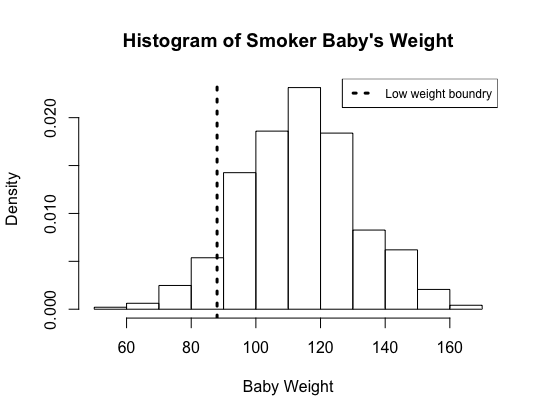
\includegraphics[width=150mm]{hist_smoker.png}

\begin{verbatim}
> summary(smoke_wt$bwt)
   Min. 1st Qu.  Median    Mean 3rd Qu.    Max. 
   58.0   102.0   115.0   114.1   126.0   163.0 
> sd(smoke_wt$bwt)
[1] 18.09895
\end{verbatim}

\newpage
\subsection*{Q5-b}
\begin{verbatim}
> low_wt_rt <- nrow(smoke_wt[baby_dt$bwt<88,]) / nrow(smoke_wt)
> low_wt_rt
[1] 0.1198347
\end{verbatim}

\noindent $11.98 \%$ of baby born to smoker mother have low birthweight. 

\subsection*{Q5-c}
\noindent Assuming number of low weight baby $X$ follows binomial distribution with probability $p$ of getting low weight. \\
\noindent $H_0$: $p = 0.03$, $H_1$: $p > 0.03$ \\
\noindent In the dataset of smoker baby weight, 58 out of 484 are low weighted.
\begin{align*}
\text{p-value} &= P(X \geq 58 | H_0) \\
&= \sum_{58}^{484} {484 \choose i}  0.03^{i} \cdot 0.97^{484-i}
\end{align*}

\noindent The sample size is large enough, so we may use normal approximation to estimate p-value. \\
\noindent $X \sim N(\mu, \sigma^2)$ \\
\noindent  where $\mu = p_0 n = 0.03 \cdot 484 = 14.52$ \\
$\sigma^2 = p_0(1-p_0)n = 0.03 * 0.97 * 484 = 14.08$  \\
\begin{align*}
\text{p-value} &= P(X \geq 58) \\
&= P(Z \geq \frac{58 - \mu }{\sqrt{\sigma^2}}) \\
&\approx 0
\end{align*}

\begin{verbatim}
> binom.test(58, 484, 0.03)$p.value
[1] 8.933056e-19
\end{verbatim}

\noindent In R, p-value is calculated as $8.933056e-19$ which is also close to 0.\\
\noindent Thus, under test size 0.05, we may reject the null, and conclude that the probability of baby getting low birthweight born to smoker mother is higher than 0.03.

\end{document}